% Template for IGARSS-2020 paper; to be used with:
%          spconf.sty  - LaTeX style file, and
%          IEEEbib.bst - IEEE bibliography style file.
% --------------------------------------------------------------------------
\documentclass{article}
\usepackage{spconf,amsmath,epsfig, physics}

\usepackage[utf8]{inputenc}
\usepackage[T2A]{fontenc}
\usepackage[english,russian]{babel}
\usepackage{microtype}
\usepackage{subcaption, caption, float}
\usepackage{cite}

\captionsetup{subrefformat=parens}
\usepackage{mathtools}

% Эта опция включает нумерацию только у тех формул,
% на которые есть ссылка в документе
\mathtoolsset{showonlyrefs=true} 

% Example definitions.
% --------------------
\def\x{{\mathbf x}}
\def\L{{\cal L}}
\newcommand\fullsum{\sum\limits_{n=1}^{N} }
\newcommand\fullphase{\omega_{n}t + \vec \kappa_{n}\vec r_0 + \psi_{n}}
\usepackage{nomencl}
\makenomenclature  

\makeatletter
    \newcommand{\whereNoStar}[2]{#1 -- #2\nomenclature{#1}{#2}}
    \newcommand{\whereStar}[2]{#1\nomenclature{#1}{#2}}
    \newcommand{\where}{
                 \@ifstar
                 \whereStar%
                 \whereNoStar%
    }
\makeatother

% Title.
% ------
%\title{Simulation the backscattered radar  cross  section measurements using
%dual-frequency radar on a model of a sharpened sea surface}
\title{Simulation measurements using Dual-frequency Precipitation Radar (DPR) on a
model of roughness sea surface}
%
% Single address.
% ---------------
\name{Kirill Ponur, Vladimir Karaev, Mariya Panfilova}
\address{Institute of Applied Physics of the Russian Academy of Sciences}
%
% For example:
% ------------
%\address{School\\
%	Department\\
%	Address}
%
% Two addresses (uncomment and modify for two-address case).
% ----------------------------------------------------------
%\twoauthors
%  {A. Author-one, B. Author-two\sthanks{Thanks to XYZ agency for funding.}}
%	{School A-B\\
%	Department A-B\\
%	Address A-B}
%  {C. Author-three, D. Author-four\sthanks{The fourth author performed the work
%	while at ...}}
%	{School C-D\\
%	Department C-D\\
%	Address C-D}
%
\begin{document}
%\ninept
%
\maketitle
%
\begin{abstract}
    В данной работе было проведено моделирование схемы измерения радиолокатора
    DPR (Dual-frequency Precipitation Radar) спутника GPM (Global Precipitation
    Measurements) на взволнованной морской поверхности. При моделировании схемы
    измерения решалась задача обратного рассеяния электромагнитного излучения.
    Для её решения искалось отраженное от зеркальных точек поле вблизи приемной
    антенны, а затем моделировалось удельное сечение обратного рассеяния и
    исследовалось его зависимость от неявных параметров: безразмерного разгона
    и направлении распространения волнения относительно движения
    спутника.
\end{abstract}
%
%\begin{keywords}

%\end{keywords}
%
\section{Introduction}
\label{sec:intro}

Моделирование морской поверхности является важным и развивающимся
направлением, но несмотря на это остается ряд вопросов, которые требуют дальнейших исследований в приложении к решаемой
задаче. 

Для описания поверхностного волнения современные модели активно применяют
уравнения гидродинамики. Наиболее известными в настоящее время являются модели
третьего поколения WAM (WaveModel), SWAN (Simulation Waves Nearshore) и
WaveWatch III \cite{wavewatch3, swan, wam4}, учитывающие взаимодействие между
четырьмя волнами и процессы обрушения волн с  образованием  пены  и  брызг.
%Для описания поверхностного волнения эти модели применяют уравнения
%гидродинамики, но в общем виде задача пока не по силам современной
%вычислительной технике. Благодаря упрощениям и предположениям задача становится
%«счетной», но требует слишком много вычислительных ресурсов, поэтому этот
%подход используется для решения научно-исследовательских задач, например,
%\cite{slunyaev2006, slunyaev2009, west1987}. 

В данной работе на модельной морской поверхности будет решаться задача
обратного рассеяния электромагнитного излучения и моделироваться схема
измерения Dual-frequency Precipitation Radar (DPR) спутника GPM. 
При её решении необходимо найти отраженное поля вблизи приемной антенны, а для
этого необходимо выполнить интегрирование по всей рассеивающей площадке.  Для
получения точного результата в результате интегрирования необходимо обеспечить
шаг по поверхности в несколько раз меньше длины волны излучения
\cite{toporkov:brown:2000, toporkov:brown:2002}. 

Для типичного пятна DPR необходимо будет построить модель поверхности размером
25 км$^2$ с разрешением порядка $0.2$ см, вычисление на такой поверхности
двумерного интеграла занимает слишком много времени на современной технике. К
тому же само моделирование поверхности такого размера является сложной задачей
для моделей, опирающихся на уравнения гидродинамики. 

Поэтому для оценки эффективности работы радиолокационной аппаратуры
больше подходит хорошо известный подход, опирающийся на модель спектра
волнения, например, \cite{longe-higgins}. В этом случае морская поверхность представляется в
виде набора гармоник, амплитуда которых вычисляется по спектру волнения. При
таком подходе смоделированная морская поверхность утрачивает ряд свойств,
присущих реальной морской поверхности, но становится более удобной для счета и
моделирование может быть проведено на за приемлемое время. Именно этот подход выбран для моделирования морской поверхности в данной работе. 

Однако смоделированная одними лишь гармоническими функциями будет симметрична
и иметь нулевое среднее. Из экспериментов 
%\cite{shuleykin} 
известно, что
настоящая морская поверхность имеет более острые вершины и пологие впадины, по
сравнению с синусоидами. Поэтому в данной работе используется модель
заостренной поверхности (CWM) \cite{nouguier}.


Надо отметить, что для выбранного подхода
качество моделирования зависит от используемого спектра волнения и от численной
реализации процедуры моделирования. Был выбран спектр \cite{ryabkova},
учитывающий короткие волны, играющие особую роль в задачах рассеяния.


\section{Model of roughness sea surface}%
\begin{figure}[t]
\centering
\makeatletter
    \@for\i:={1,2,3}\do{
    \begin{subfigure}{0.45\linewidth}
        \centering
        \includegraphics[width=\linewidth, page=\i]{figs/cwm_demo_1d_igarss}
        \subcaption{}
        \label{subfig:cwm_modeling\i}
    \end{subfigure}
    %\hfill
}


\caption{
    \subref{subfig:cwm_modeling1} поле высот;
    \subref{subfig:cwm_modeling2} поле наклонов вдоль направления
    распространения волнения;
    \subref{subfig:cwm_modeling3} поле наклонов перпендикулярное направлению
    распространения волнения;
    Синей линией отмечена обычная поверхность, оранжевой -- заостренная.
    Полностью развитое волнение $\tilde x = 20170$, скорость ветра $U_{10} = 5
    $ м/с.
}

\makeatother
\label{fig:cwm_modeling}
\end{figure}

Обычный способ моделирования морской поверхности по известному спектру волнения
заключается в суммировании гармоник с детерменированными амплитудами и
случайными фазами. Поле возвышений в этом случае \where*{$\zeta$}{поле
возвышений} представляется в виде
\begin{equation}
    \label{eq:surface3d_default}
    \zeta(\vec r, t) = \fullsum A_n(\vec \kappa_{nm}) \cos(\fullphase),    \\
\end{equation}
где \where{$\vec \kappa$}{двумерный волновой вектор},  
$\vec r_0 = (x_0, y_0)$, $\vec r = (x, y)$, 
\where{$\psi_{nm}$}{случайная фаза равномерно распределенная в интервале от $0$ до $2 \pi$}, 

\where{$A_n (\vec \kappa_n)$}{амплитуда гармоники с волновым
вектором}, вычисляемая по известному спектру волнения \cite{ryabkova},
$\vec \kappa_n$ и временной частотой
\where*{$\omega_n(\kappa_{nm})$}{дисперсионное соотношение}.%\cite{pustovoytenko}.


Для перехода к модели заостренной поверхности необходимо ввести следующие
преобразования координат \cite{nouguier}, тем самым превращая моделирование
независимыми гармоническими функциями в моделирование трохоидами
\begin{equation}
    \begin{gathered}
        \label{eq:surface3d_cwm}
        x(\vec r,t) = x_0 - \fullsum A_n(\vec \kappa_{n})\frac{\vec \kappa_x}{\kappa}        \sin(\fullphase)\\
        y(\vec r,t) = y_0 - \fullsum A_n(\vec \kappa_{n}) \frac{\vec \kappa_y}{\kappa}
        \sin(\fullphase)\\
    \end{gathered}
\end{equation}

Сравнение основных характеристик обычной и заостренной морской поверхности
приведено на рис. \ref{fig:cwm_modeling}.

%Наклоны поверхности в каждой точке можно найти дифференцируя
%\eqref{eq:surface3d_cwm} 
%\begin{equation}
    %\begin{gathered}
        %\xi_{x}(\vec r,t) = \pdv{\zeta(\vec r,t)}{x_0} = \fullsum \kappa_{x} A_n(\vec \kappa_{nm}) \cdot \sin(\fullphase)    \\
        %\xi_{y}(\vec r,t) = \pdv{\zeta(\vec r,t)}{y_0} = \fullsum  \kappa_{y} A_n(\vec \kappa_{nm}) \cdot \sin(\fullphase)    \\
    %\end{gathered}
%\end{equation}



\section{Scattering model}%

%В данной работе будет проводиться айти УЭПР в зависимости от углов падения.
%Чтобы найти $\sigma$ ЭПР морской поверхности её для начала придется вычислить по
%определению ЭПР 
%\begin{equation}
    %\sigma = 4 \pi R^2 \abs{\frac{E_2^2}{E_1^2}}
%\end{equation}

%Поле отраженной от поверхности сферической волны можно вычислить,
%интегрируя по всей отражающей площадке $S$
%\begin{equation}
    %E_2 = \frac{1}{\lambda} \int\limits_{S} \frac{E_1}{R} G(\theta, \phi) \exp(-j \cdot 2 k R)
    %\cos \theta \dd S,
%\end{equation}
%где $R$ -- расстояние от антенны до точки на площадке. 

%%\begin{equation}
    %%\frac{E_2}{E_1} = \frac{1}{\lambda} \exp(-j \cdot 2k R_0)
    %%\int\limits_{S} \frac{1}{R} \exp{-j \cdot 2 k r } \dd S
%%\end{equation}

%\begin{equation}
    %\label{eq:sigma}
    %\sigma = \frac{4 \pi R^2}{\lambda^2} \abs{\int\limits_{S}^{} \frac{G(\theta,
            %\phi)}{R} \exp{-j \cdot 2 k
    %r } \cos \theta \dd S}^2
%\end{equation}

%Мы же будем работать с УЭПР, определяемой следующим образом
%\begin{equation}
    %\label{eq:crosssec}
    %\sigma_0 =   \sigma \cdot \qty(\int\limits_S G(\theta, \phi) \dd S)^{-1},
%\end{equation}
%где $G(\theta, \phi)$ -- диаграмма направленности антенны.

Для точного вычисления УЭПР для всей морской поверхности слишком сложно и
ресурсоемко, поскольку её точное вычисление требует счета двумерного интеграла
по всей рассеивающей площадке.  

Однако при малых углах падения, при которых
работает DPR, основной вклад вносит механизм зеркального отражения, поэтому мы
будем считать УЭПР только от точек, дающих максимальный вклад в отраженный
сигнал. %-- тех, для которых максимально скалярное произведение вектор $\vec R$ и
%нормали к поверхности в текущей точке  $\vec n$: для зеркальных точек. 

%Искать
%все зеркальные точки мы тоже не в состоянии, поэтому будем искать только точки
%из достаточно большой выборки. Если выборка получится достаточно большой, то
%разницы между практикой не будет. 

Математически, мы заменяем интеграл по всей рассеивающей поверхности на
сумму по выборке зеркальных точек. В случае достаточно большой выборки
зеркальных точек для гауссовой морской
поверхности будет мы получим распределение, совпадающее с теорией
\begin{equation}
    \label{eq:sigma0_theory}
    \sigma_0 = \frac{\abs{F(0)}^2}{\cos^4\theta \sqrt{\sigma_{xx}^2
    \sigma_{yy}^2 - K_{xy}^2(0)}} \exp{- \frac{\sigma^2_{xx}
    \tan^2\theta}{\sigma_{xx}^2 \sigma_{yy}^2 - K_{xy}^2(0)}}
\end{equation}

%Спутник DPR работает в двух диапазонах, имеющих различные дисперсии наклонов.
%Поскольку Ka-диапазон имеет волну, короче, чем Ku-диапазон, то в нём мы сможем
%увидеть больше неровностей морской поверхности и меньшее количество зеркальных
%площадок. Поэтому в Ka-диапазоне УЭПР при нулевом угле падения будет меньше,
%чем в Ku-диапазоне.  Этот эффект предсказывает и теоретическая формула
%\eqref{eq:sigma0_theory}. 
%Распределение зеркальных точек в двух диапазонах для антенны, направленной
%вертикально вниз представлено на рис. \ref{fig:mirror_dots_distrib}. 
%Зеркальные точки при нулевом угле падения должны располагаться преимущественно
%на пиках и впадинах поверхности, практически отсутствуя на склонах. Это также
%отражает рис. \ref{fig:mirror_dots_distrib}.

%Для выборки зеркальных точек  интеграл \eqref{eq:sigma} разбивается на сумму
%площадей отдельных зеркальных площадок. 


%\begin{figure}[h]
    %\centering
    %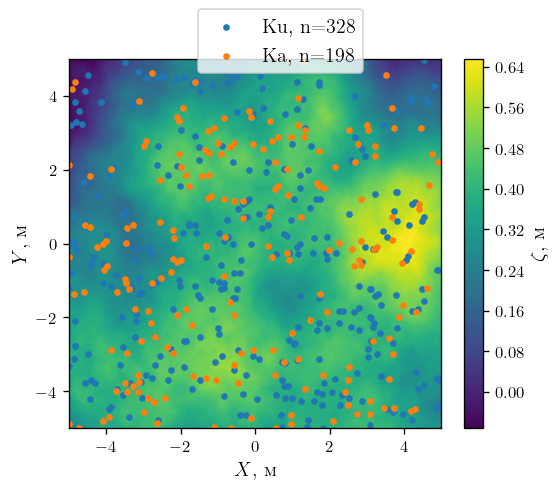
\includegraphics[width=0.6\linewidth]{figs/mirrordots.png}
    %\caption{Распределение зеркальных точек на двумерной поверхности высот для
    %Ku- и Ka-диапазонов, $n$--количество соответствующих точек на поверхности }
    %\label{fig:mirror_dots_distrib}
%\end{figure}

Для валидации модели были получены данные спутника  и произведено сравнение
срезов трека с модельными данными в Ku-диапазоне (см. рис. \ref{fig:crosssec}).

Поскольку при моделировании учитывалось только зеркальное отражение и
исключалось влияние брэгговского рассеяния, то это
позволяет производить моделирование при углах отклонения антенны более чем $12^\circ$. 


\begin{figure}[t]
    \centering
    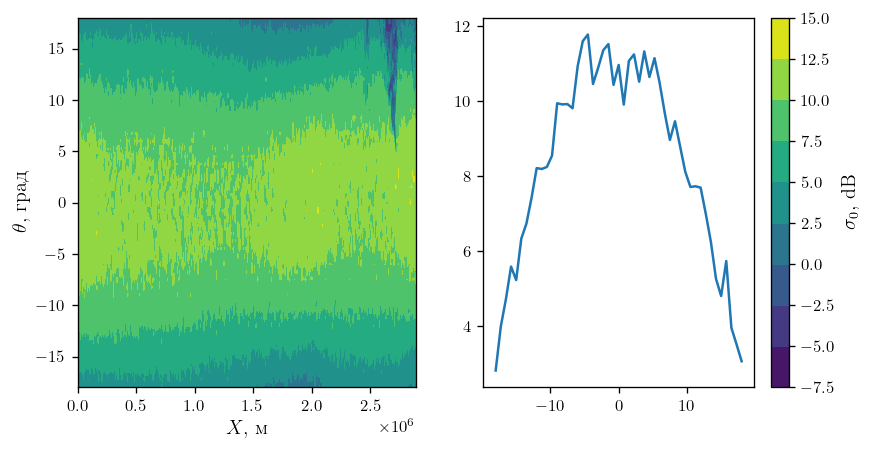
\includegraphics[width=0.6\linewidth]{figs/real_crosssec.png}
    \caption{Зависимость УЭПР $\sigma_0$ от угла падения  $\theta$; 
    черной линией обозначено теоретическое значение УЭПР,
    крестиками -- значение, полученное по данным DPR,
    кружочками -- значение, посчитанное по срезу обычной морской поверхности,
    треугольниками -- значение, посчитанное по срезу заостренной морской поверхности
}
    \label{fig:crosssec}
\end{figure}






%Из рис. \ref{fig:crosssec} заметно, что УЭПР, полученная со спутника при росте
%угла падения начинает различаться с теоретической \eqref{eq:crosssec}. 
%Однако при моделировании заостренной поверхности мы можем точнее приблизить
%модельную кривую к реальной

%\footnote{Усреднить модельные кривые за 100 срезов,
%чтобы выглядело красивее}
%\begin{figure}[t]
    %\centering
    %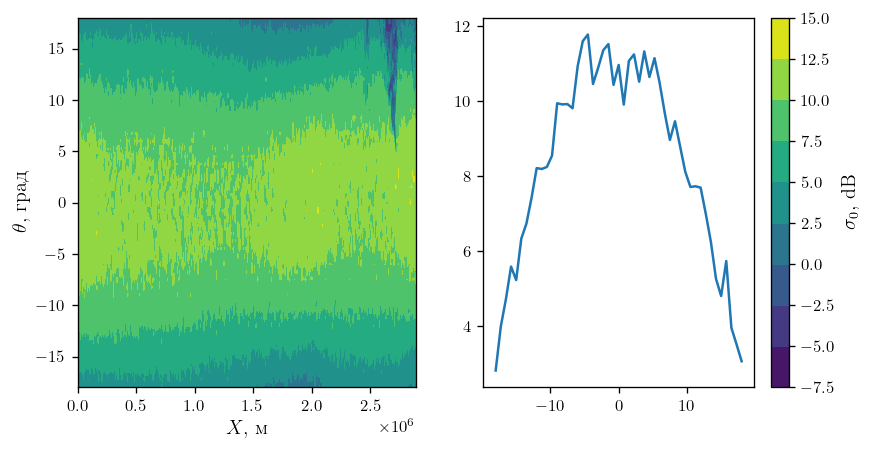
\includegraphics[width=0.8\linewidth]{figs/real_crosssec.png}
    %\caption{Трек, полученный с DPR}
    %\label{fig:track_dpr}
%\end{figure}




\section{Numerical experiment with DPR in Ku-band}%

С помощью предложенной модели взволнованной морской поверхности был поставлен
численный эксперимент и исследованы зависимости УЭПР от безразмерного разгона
волнения и направлении распространения волнения относительно движения
спутника.

На рис.  \ref{scap:crosssec_slices:1} представлена симуляция трека DPR при
скорости приводного ветра $U_{10}=7$ м/с и меняющемся безразмерном разгоне
волнения. Одномерные срезы панорамного
изображения  представлены на рис. \ref{scap:crosssec_direction:2},
\ref{scap:crosssec_direction:3}. Результат моделирования несложно
интерпретировать: увеличение разгона <<сглаживает>> морскую поверхность, убирая
коротковолновую составляющую спектра, поэтому при надирном зондировании УЭПР
развитого волнения немного превосходит УЭПР развивающегося. 
Также, увеличивающийся разгон делает поверхность более пологой
из-за увеличении длин доминантных волн, в результате
для средних углов падения  $\theta > 15^{\circ}$  зеркальных площадок
становится меньше и УЭПР уменьшается. 


Более интересная зависимость представлена на рис.
\ref{scap:crosssec_direction:1}, построенном при скорости приводного ветра $U_{10}=7$ м/с и меняющемся направлении распространения волнения
$\phi_0$ относительно движения спутника. Одномерные срезы панорамного
изображения  представлены на рис. \ref{scap:crosssec_direction:2},
\ref{scap:crosssec_direction:3}. На рис. \ref{scap:crosssec_direction:2} видно,
что при малых углах наблюдения морская поверхность для радиолокатора выглядит
почти одинаково вне зависимости от направления волнения, однако с увеличением
угла наблюдения большую роль играет дисперсия наклонов вдоль направления
зондирования $\sigma_yy^2$, а она принимает минимальные значения при
$\phi_0=0^{\circ}$  и максимальные при $\phi_0 = 90^{\circ}$. 

\begin{figure}[t]
    \centering
    \begin{subfigure}{\linewidth}
        \centering
        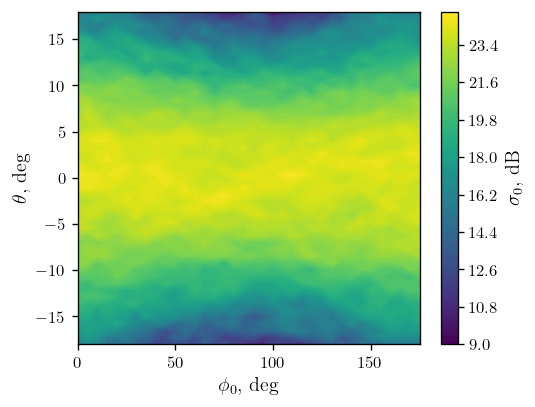
\includegraphics[width=0.8\linewidth]{figs/direction.png}
        \caption{}
        \label{scap:crosssec_direction:1}
    \end{subfigure}

    \begin{subfigure}{\linewidth}
        \centering
        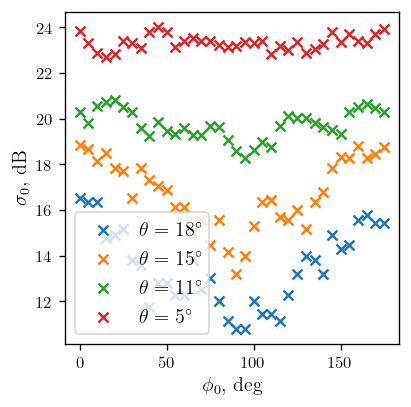
\includegraphics[width=0.6\linewidth]{figs/direction_slices1.png}
        \caption{}
        \label{scap:crosssec_direction:2}
    \end{subfigure}

    \begin{subfigure}{\linewidth}
        \centering
        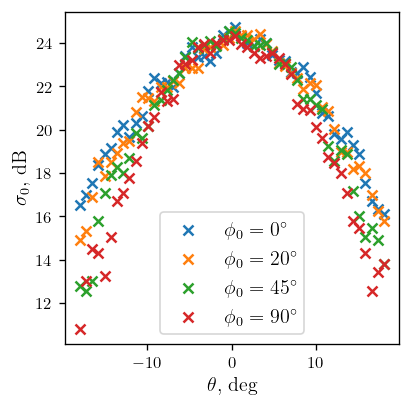
\includegraphics[width=0.6\linewidth]{figs/direction_slices.png}
        \caption{}
        \label{scap:crosssec_direction:3}
    \end{subfigure}
    \caption{
    Моделирование трека DPR на взволнованной морской поверхности при
        скорости ветра $U_{10}=7$ м/с.
        \subref{scap:crosssec_direction:1} Панорамное изображение УЭПР в
        зависимости от направления распространения волнения $\phi_0$ и
        угла отклонения антенны от надира
        \\
        \subref{scap:crosssec_direction:2} Срез панорамного изображения
        вдоль фиксированного отклонения антенны
        \\
        \subref{scap:crosssec_direction:3} Срез панорамного изображения
        вдоль фиксированного направления распространения волнения
    }
    \label{fig:crosssec_clices}
\end{figure}

\begin{figure}[t]
    \centering
    \begin{subfigure}{\linewidth}
        \centering
        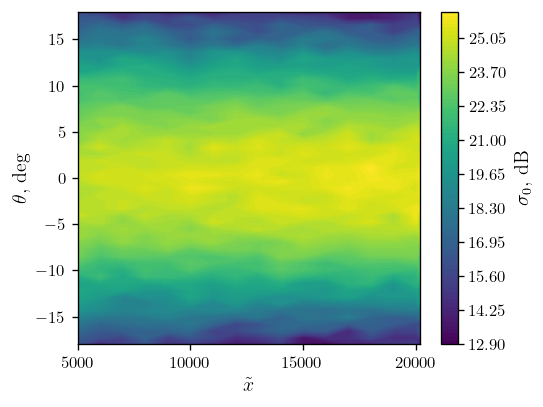
\includegraphics[width=0.8\linewidth]{figs/fetch.png}
        \caption{}
        \label{scap:crosssec_slices:1}
    \end{subfigure}
    \begin{subfigure}{\linewidth}
        \centering
        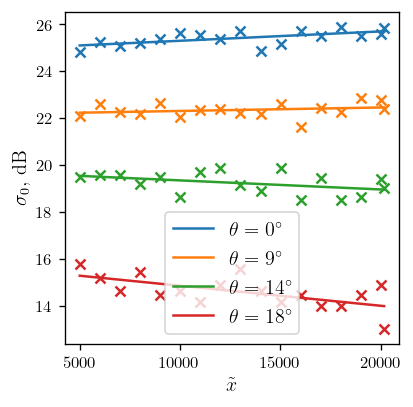
\includegraphics[width=0.6\linewidth]{figs/fetch_slices.png}
        \caption{}
        \label{scap:crosssec_slices:2}
    \end{subfigure}

    \begin{subfigure}{\linewidth}
        \centering
        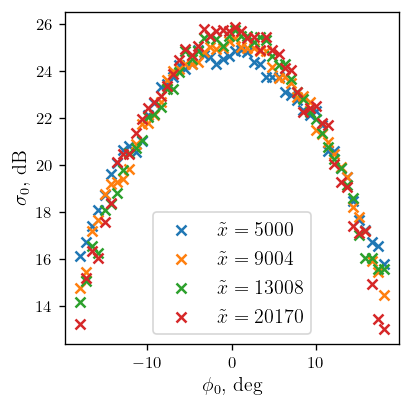
\includegraphics[width=0.6\linewidth]{figs/fetch_slices1.png}
        \caption{}
        \label{scap:crosssec_slices:3}
    \end{subfigure}
    \caption{
    Моделирование трека DPR на взволнованной морской поверхности при
        скорости ветра $U_{10}=7$ м/с.
        \subref{scap:crosssec_slices:1} Панорамное изображение УЭПР в
        зависимости от безразмерного разгона ветрового волнения $\tilde x$ и
        угла отклонения антенны от надира
        \\
        \subref{scap:crosssec_slices:2} Срез панорамного изображения
        вдоль фиксированного отклонения антенны
        \\
        \subref{scap:crosssec_slices:3} Срез панорамного изображения
        вдоль фиксированного значения безразмерного разгона волнения
    }


    \label{fig:crosssec_clices}
\end{figure}



\section{Conclusion}

В данной работе было проведено моделирование схемы измерения DPR спутника GPM
на взволнованной морской поверхности. При моделировании схемы измерения 
решалась задача обратного рассеяния электромагнитного излучения. Для её решения искалось отраженное от зеркальных точек поле вблизи приемной антенны, а затем
моделировалось удельное сечение обратного рассеяния.

Морская поверхность представляла собой
сумму независимых трохоид со случайными фазами, амплитуда которых вычислялась
по известному спектру волнения. Для оценки работоспособности модели было
проведено сравнение с данными радиолокатора DPR проекта Global Precipitation
Measurements (GPM). В пределах углов отклонения антенны от надира $\theta \leq
\pm 12^{\circ}$ построенная модель хорошо согласуется с теорией и полученными
экспериментальными данными.


\textbf{This work   was   funded   by   the   Russian   Science Foundation
(Project RSF 20-17-00179). The DPR data are presented  by  the  JAXA  (JAXA
Satellite  Project  Research (Non-Funded)PI  N ER2GPN108).}


% References should be produced using the bibtex program from suitable
% BiBTeX files (here: strings, refs, manuals). The IEEEbib.bst bibliography
% style file from IEEE produces unsorted bibliography list.
% -------------------------------------------------------------------------
\newpage
\bibliographystyle{IEEEbib}
\bibliography{main}


\end{document}
